\documentclass{standalone}
\usepackage{tikz}
\usepackage{amssymb}

\begin{document}
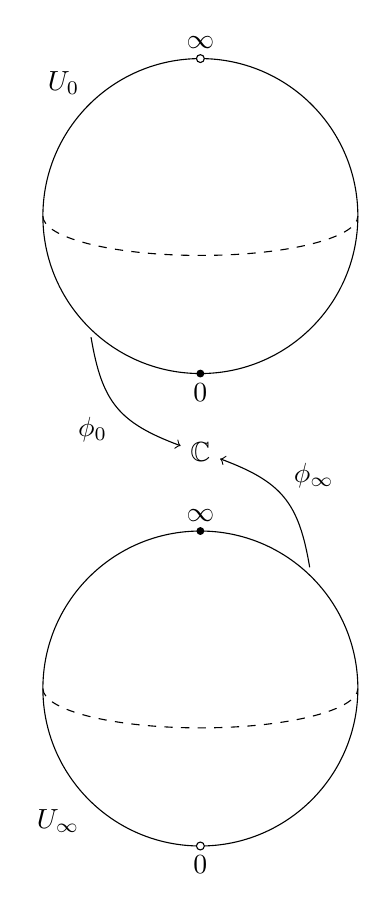
\begin{tikzpicture}
	\begin{scope}[yshift=-3cm]
		\draw (0,0) circle (2);
		\draw[dashed] (-2,0) arc[start angle=-180, end angle=0, x radius=2, y
				radius=0.5];
		\node[below left] at (-135:2){$ U _{\infty} $};
		\fill (0,2) circle (0.05) node[above]{$ \infty $};
		\filldraw[fill=white] (0,-2) circle (0.05) node[below]{$ 0 $};
		\node (t) at (45:2){};
	\end{scope}

	\begin{scope}[yshift=3cm]
		\draw (0,0) circle (2);
		\draw[dashed] (-2,0) arc[start angle=-180, end angle=0, x radius=2, y
				radius=0.5];
		\node[above left] at (135:2){$ U _{0} $};
		\filldraw[fill=white] (0,2) circle (0.05) node[above]{$ \infty $};
		\fill (0,-2) circle (0.05) node[below]{$ 0 $};
		\node (b) at (-135:2){};
	\end{scope}

	\node (C) at (0,0){$ \mathbb{C} $};

	\draw[bend right, ->, looseness=1.2] (b) to node[below left]{$ \phi_0 $} (C);
	\draw[bend right, ->, looseness=1.2] (t) to node[above right]{$ \phi _{\infty} $} (C);
\end{tikzpicture}
\end{document}

